\subsection{Anomaly detection approach}

In order to measure the performance of any anomaly detection techniques, we need a labelled dataset. Tagging anomalous points in gene expression time series manually is a tiresome task and needs expert suggestion. Therefore, with the unavailability of labelled data, we have to use some statistical method designed for time series to fit entire series and identify anomaly points from them. Then we apply some unsupervised and supervised machine learning based approach to detect anomaly and compare their performance using the labelled data. Our experiment runs on three real dataset basic, ccycle and yeast. The details of the dataset are described in experiment section. 

\subsubsection{Statistical method for anomaly labelling}
We use moving average, weighted moving average, exponential smoothing, double exponential smoothing methods to fit the entire time series of individual genes. For a gene $g$ and its time series $g_T$, any time point $x_t \in g_T$ is said to be anomalous if $|x_t-x'_t|> \delta$; where $\delta$ is the threshold and $x'_t$ is the expected value computed by statistical method. The choice of $\delta$ is dependent of dataset and set by trail and error. We assume that most of the points of time series gene expression are normal and only a few points ($<10\%$) are considered to be anomalous. Figure \ref{fig:stat_basic}, \ref{fig:stat_ccycle}, \ref{fig:stat_yeast} show the effect of each methods in all three dataset.

\begin{figure*}[h]
	\centering
	\begin{subfigure}[b]{0.48\textwidth}
		\centering
		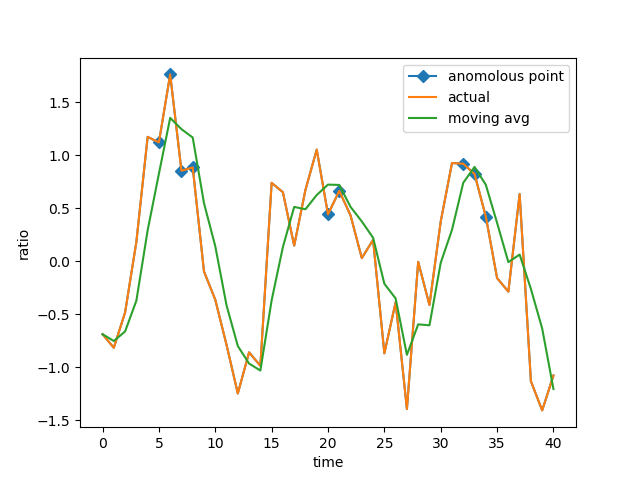
\includegraphics[width=\textwidth]{stat_fig/basic_moving_avg.png}
	\end{subfigure}
	\hfill
	\begin{subfigure}[b]{0.48\textwidth}  
	    \centering 
	    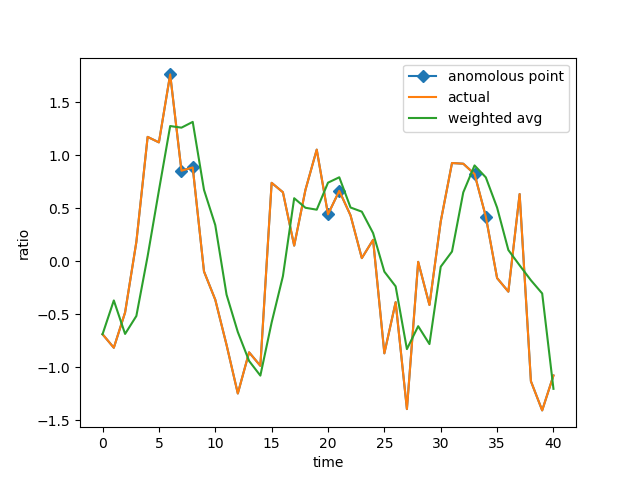
\includegraphics[width=\textwidth]{stat_fig/basic_weighted_avg.png}
	\end{subfigure}
	\vskip\baselineskip
	\begin{subfigure}[b]{0.48\textwidth}   
		\centering 
		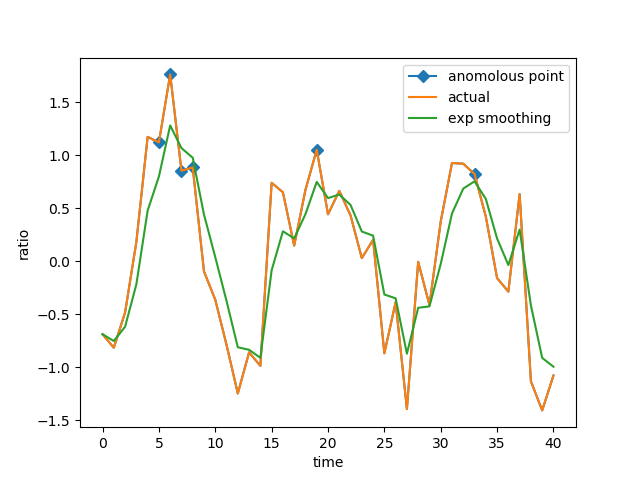
\includegraphics[width=\textwidth]{stat_fig/basic_exp.png}
	\end{subfigure}
	\quad
	\begin{subfigure}[b]{0.48\textwidth}   
		\centering 
		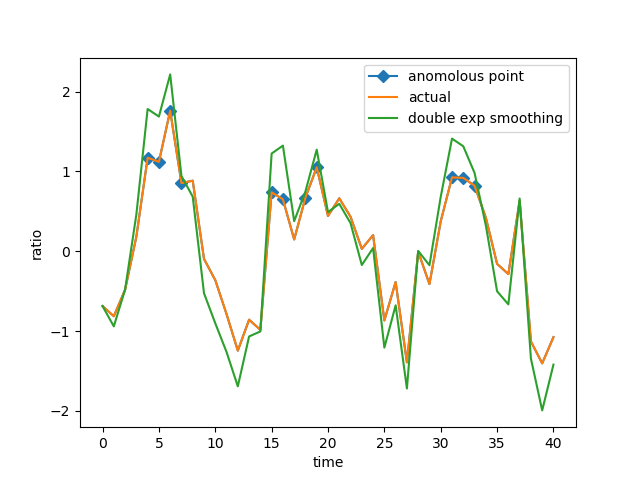
\includegraphics[width=\textwidth]{stat_fig/basic_double_exp.png}		
	\end{subfigure}
	\caption{Statistical methods applied on a sample gene of basic dataset}
	\label{fig:stat_basic}
\end{figure*}
\paragraph*{\textbf{Moving Average}}
The first step in a classical decomposition is to use a moving average method to estimate the trend-cycle of a time series. Predicted value of $t$ instance of a moving average of order $m$ can be written as,
\begin{align*}
    x'_t &= \frac{1}{m}\sum_{i=1}^{m}x'_{t-i} \\
    x'_t &= x_t ; t=1,2,\dots m
\end{align*}
Here, optimal value of $m$ depends on the trend cycle length and is set by trail and error according to dataset. For our experiment it is set to be $3$.

\paragraph*{\textbf{Weighted moving Average}}
Simple moving average considers each previous values as equally weighted. The combination of different weights of previous values provide a weighted moving average form. Predicted value of $t$ instance of a weighted moving average of order $m$ can be written as,
\begin{align*}
    x'_t &= \frac{1}{m}\sum_{i=1}^{m}w_ix'_{t-i} \\
    x'_t &= x_t ; t=1,2,\dots m
\end{align*}
Here, $w_1, w_2, \dots w_m$ are the weights of previous $m$ time points respectively and $\sum_{i=1}^{m}w_i=1$. In our experiment, weights are set as $0.5, 0.3, 0.2$ for 3  window moving average procedure.
\begin{figure*}[h]
	\centering
	\begin{subfigure}[b]{0.48\textwidth}
		\centering
		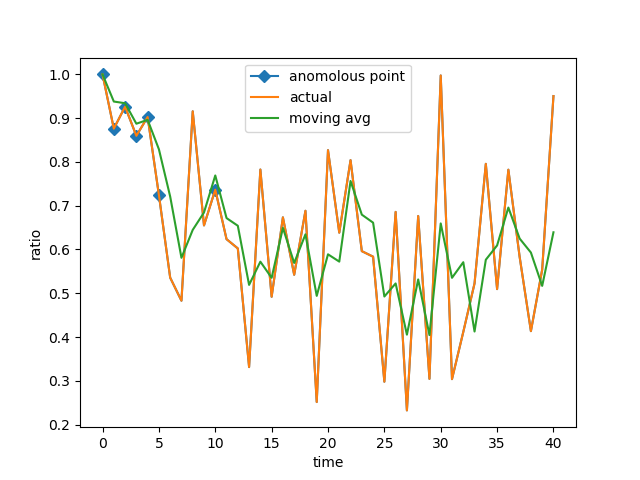
\includegraphics[width=\textwidth]{stat_fig/ccycle_moving_avg.png}
	\end{subfigure}
	\hfill
	\begin{subfigure}[b]{0.48\textwidth}  
	    \centering 
	    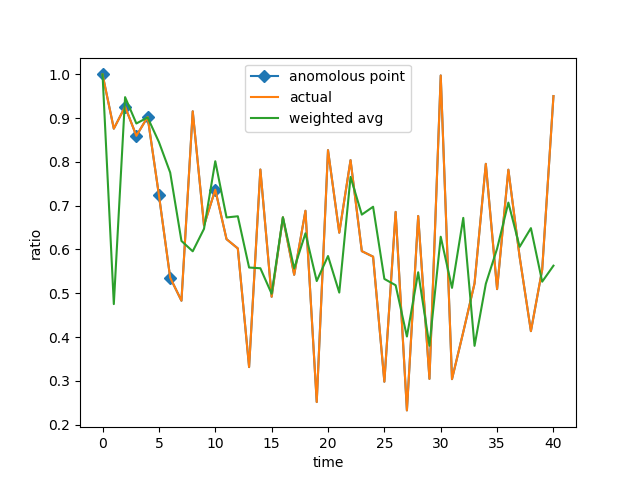
\includegraphics[width=\textwidth]{stat_fig/ccycle_weighted_avg.png}
	\end{subfigure}
	\vskip\baselineskip
	\begin{subfigure}[b]{0.48\textwidth}   
		\centering 
		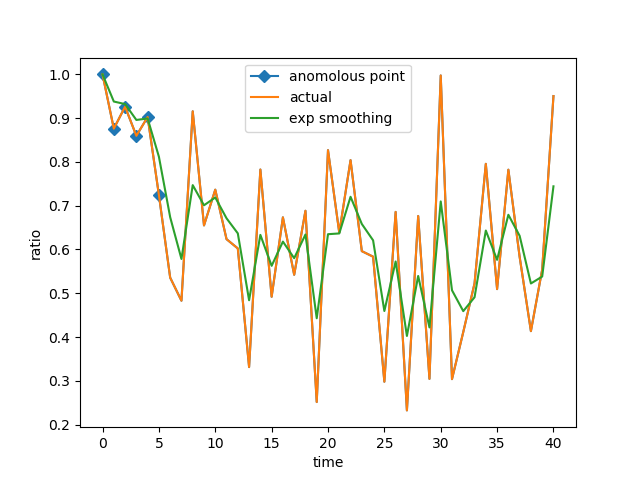
\includegraphics[width=\textwidth]{stat_fig/ccycle_exp.png}
	\end{subfigure}
	\quad
	\begin{subfigure}[b]{0.48\textwidth}   
		\centering 
		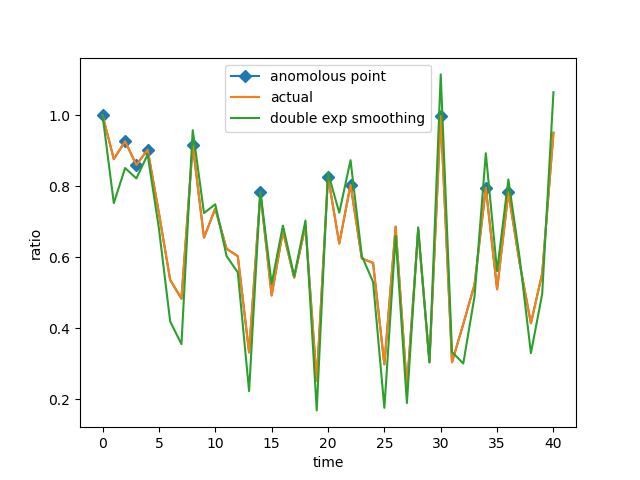
\includegraphics[width=\textwidth]{stat_fig/ccycle_double_exp.png}		
	\end{subfigure}
	\caption{Statistical methods applied on a sample gene of ccycle dataset}
	\label{fig:stat_ccycle}
\end{figure*}
\paragraph*{\textbf{Exponential smoothing}}
Exponential smoothing is a rule of thumb technique for smoothing time series data using the exponential window function. Whereas in the simple moving average the past observations are weighted equally, exponential functions are used to assign exponentially decreasing weights over time.
Predicted value $x'_t$ of $t$ time instance can be computed by following formula.
\begin{align*}
    x'_t &= \alpha x_t + (1-\alpha)x'_{t-1}; t>1  \\
    x'_1 &= x_1
\end{align*}
Where $\alpha$ is the smoothing factor and $0<\alpha<1$. We set $\alpha$ according to dataset and time series structure of a gene.
\paragraph*{\textbf{Double exponential smoothing}}
Simple exponential smoothing does not do well when there is a trend in the data, which is inconvenient. Although time series gene data do not suppose to follow any specific trend or seasonality, we try to apply this technique in fitting the series and fins satisfactory result.
Let $b_t$ be the best trend estimation of time $t$, then the expected value of time series $x'_t$ is calculated by following formula.
\begin{align*}
    x'_t &= \alpha x_t + (1-\alpha)(x'_{t-1}+b_{t-1}); t>2  \\
    b_t &= \beta(x'_t-x'_{t-1}) + (1-\beta)b_{t-1}; t>2  \\
    x'_2 &= x_2 \\
    x'_1 &= x_1 \\
    b_2 &= x_2 - x_1
\end{align*}
Where $\alpha$ is the data smoothing factor, $\beta$ is the trend smoothing factor and both $0<\alpha,\beta<1$. The choice of $b_1$ is a matter of preference.

\begin{figure*}[h]
	\centering
	\begin{subfigure}[b]{0.48\textwidth}
		\centering
		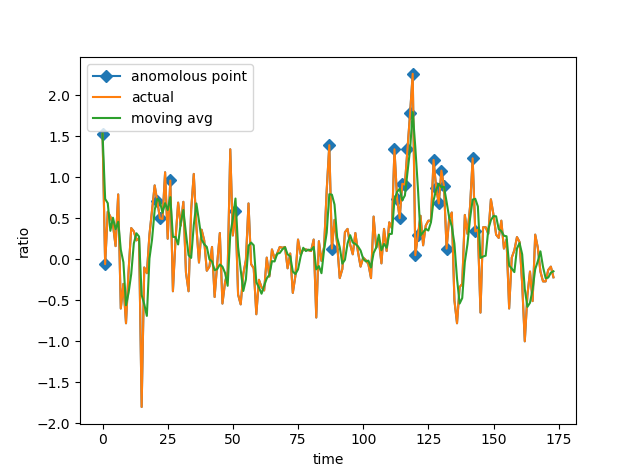
\includegraphics[width=\textwidth]{stat_fig/yeast_moving_avg.png}
	\end{subfigure}
	\hfill
	\begin{subfigure}[b]{0.48\textwidth}  
	    \centering 
	    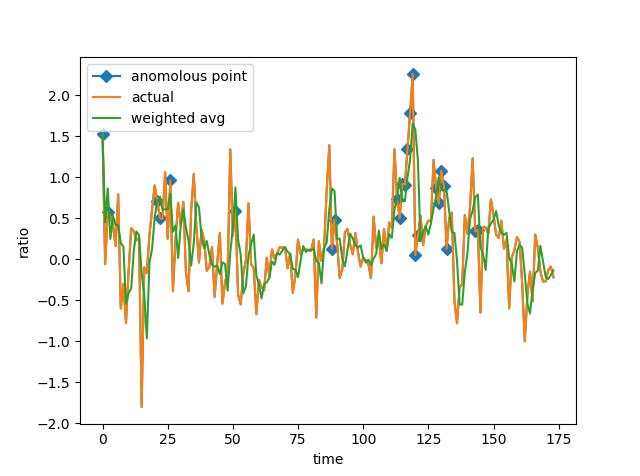
\includegraphics[width=\textwidth]{stat_fig/yeast_weighted_avg.png}
	\end{subfigure}
	\vskip\baselineskip
	\begin{subfigure}[b]{0.48\textwidth}   
		\centering 
		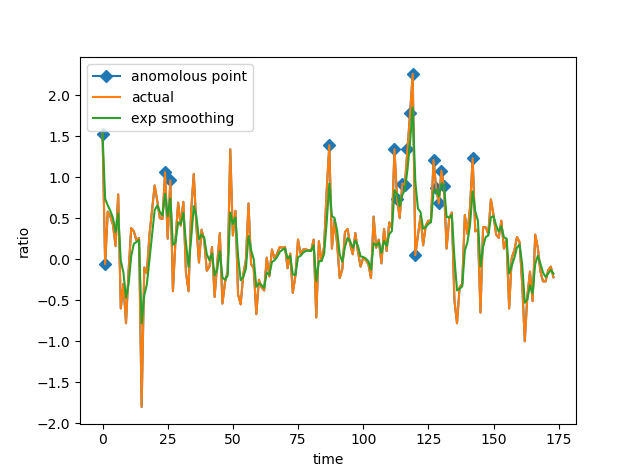
\includegraphics[width=\textwidth]{stat_fig/yeast_exp.png}
	\end{subfigure}
	\quad
	\begin{subfigure}[b]{0.48\textwidth}   
		\centering 
		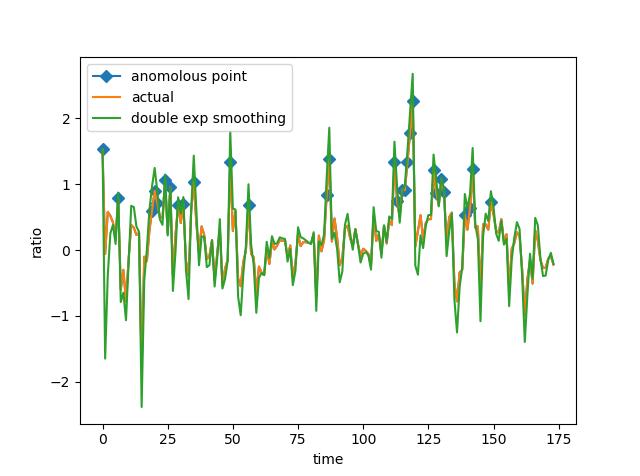
\includegraphics[width=\textwidth]{stat_fig/yeast_double_exp.png}		
	\end{subfigure}
	\caption{Statistical methods applied on a sample gene of yeast dataset}
	\label{fig:stat_yeast}
\end{figure*}
\paragraph*{\textbf{Anomaly labelling:}} Each of the method is applied for every gene of the dataset. The detailed performance of the methods is described in experiment section. For a time series each point is labelled as 0(normal) or 1(anomalous) by a method. Therefore, we aggregate the result of four methods by taking their sum and normalize them. Therefore, each data point has a score between $\{0,.25,.5,75,1\}$. 

We also take weighted sum from the output of each methods and provide a simple two class classification. A point is classified as anomalous if its score is greater than 0.5 and normal otherwise. We perform the efficiency of different methods by using both five class score based and two class classification.


\subsubsection{Unsupervised machine learning method}
Anomalous points are considered to be outlier of a distribution ina vector space. Therefore we try to apply novelty  and outlier detection algorithm in our time series gene expression.
We apply four machine learning approaches: one class support vector machine(SVM), isolation forest, local outlier factor and elliptic envelop. 

Each  method  take time series of a gene as input and classify each time point as normal or anomalous. For these methods each time point need to be represented as a feature vector. Therefore first we describe the conversation of time series in vector space and then present brief overview of these methods. Detailed performance of these methods are described in experiment section.

\paragraph{\textbf{Convert time series in vector space:}}   The
most straightforward way is to unfold the time-series into a
phase space using a time-delay embedding process. Therefore, if we want to fold a time point $x_t$ into $d$ dimensional vector space $\bm{x_t}$, then it is represented as follows.
\begin{align*}
    \bm{x_t} = [x_{t-d+1}, x_{t-d+2},\dots x_{t-1},x_t]; t=d,\dots,T
\end{align*}
But According to \cite{svm}, in some cases, when a time series is mostly composed of
low frequency components, the phase space is the set of
vectors converted from this time series distribute along the
diagonal vector $\bm{1}$, where $\bm{1}=[1,1,,\dots,1]^T$. Therefore, the concept of
\textit{projected phase space} is introduced to cope with this bias. The basic idea is to project all the vectors in a phase space
to a subspace orthogonal to the diagonal vector $\bm{1}$. That is,
according to the projection theorem,
\begin{align*}
    \bm{x'_t}=(\bm{I}-\frac{1}{d}\bm{1}\bm{1}^T)\bm{x_t}
\end{align*}

We use both normal and projected phase space in the experiment. 

\begin{figure*}[h]
	\centering
	\begin{subfigure}[b]{0.48\textwidth}
		\centering
		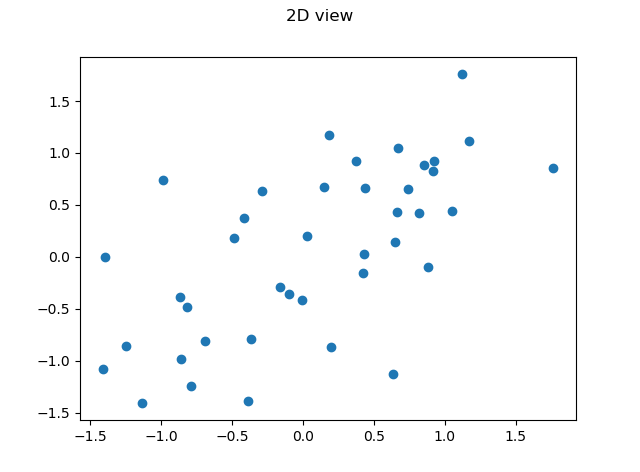
\includegraphics[width=0.75\textwidth]{vec_fig/2DnormalProject.png}
		\caption{normal vector space in 2D}
	\end{subfigure}
	\hfill
	\begin{subfigure}[b]{0.48\textwidth}  
	    \centering 
	    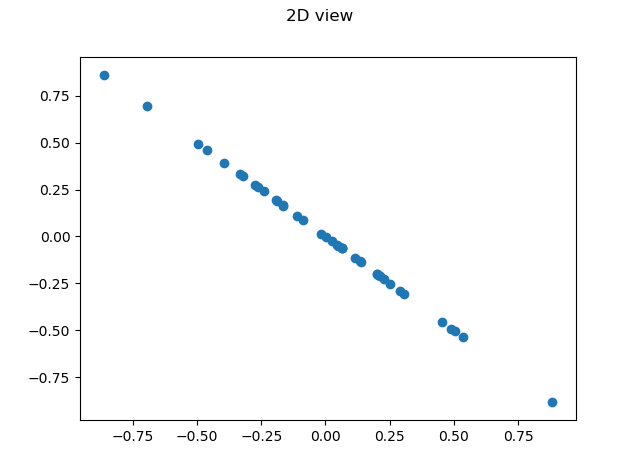
\includegraphics[width=0.75\textwidth]{vec_fig/2DdiagonalProject.png}
	    \caption{projected vector space in 2D}
	\end{subfigure}
	\vskip\baselineskip
	\begin{subfigure}[b]{0.48\textwidth}   
		\centering 
		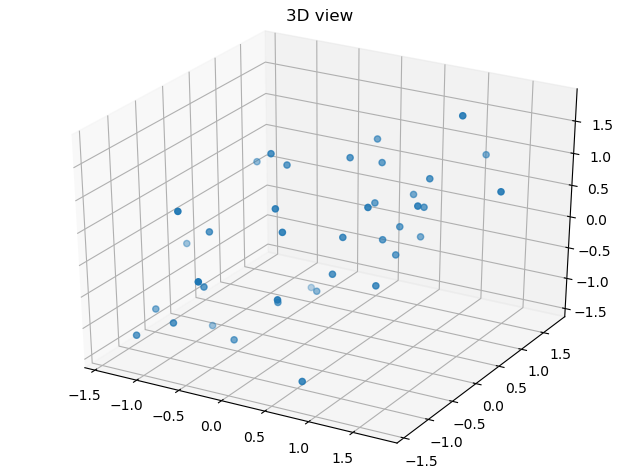
\includegraphics[width=0.75\textwidth]{vec_fig/3DnormalProject.png}
		\caption{normal vector space in 3D}
	\end{subfigure}
	\quad
	\begin{subfigure}[b]{0.48\textwidth}   
		\centering 
		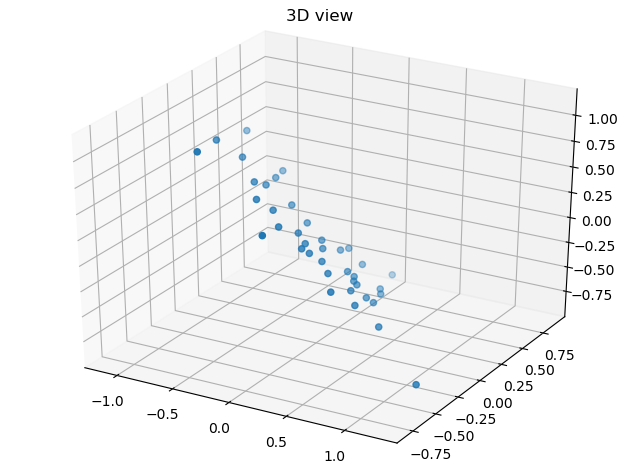
\includegraphics[width=0.75\textwidth]{vec_fig/3DdiagonalProject.png}	
		\caption{projected vector space in 3D}
	\end{subfigure}
	\caption{Vector space of time series of a gene}
	\label{fig:stat_yeast}
\end{figure*}

\paragraph*{\textbf{One class SVM}}
One-Class SVM has been introduced by Schölkopf et al.\cite{one_svm}.
It tries to learn a rough, close frontier delimiting the contour of the initial observations distribution, plotted in embedding d-dimensional space. Then, if further observations lay within the frontier-delimited subspace, they are considered as coming from the same population than the initial observations. Otherwise, if they lay outside the frontier, we can say that they are anomaly with a given confidence in our assessment.

 It requires the choice of a kernel and a scalar parameter $\nu$ to define a frontier.  The $\nu$ parameter, also known as the margin of the One-Class SVM, corresponds to the probability of finding a new, but regular, observation outside the frontier. We use the default RBF kernel and set $\nu$ to 0.1.


\paragraph*{\textbf{Isolation forest}}
The IsolationForest \cite{isolation} ‘isolates’ observations by randomly selecting a feature and then randomly selecting a split value between the maximum and minimum values of the selected feature.

Since recursive partitioning can be represented by a tree structure, the number of splittings required to isolate a sample is equivalent to the path length from the root node to the terminating node.
This path length, averaged over a forest of such random trees, is a measure of normality and our decision function.

Random partitioning produces noticeable shorter paths for anomalies. Hence, when a forest of random trees collectively produce shorter path lengths for particular samples, they are highly likely to be anomalies.


\paragraph*{\textbf{Local outlier factor}}
Breunig et al.\cite{local} present the LOF algorithm that is an unsupervised outlier detection method which computes the local density deviation of a given data point with respect to its neighbors. It considers as outlier or anaomalous samples that have a substantially lower density than their neighbors.

This algorithm takes number of neighbour points as parameter. While choosing we should consider follwing two conditions 1) greater than the minimum number of objects a cluster has to contain, so that other objects can be local outliers relative to this cluster, and 2) smaller than the maximum number of close by objects that can potentially be local outliers. We perform the experiment by taking $n\_neighbour$ to be the half of total points.


\paragraph*{\textbf{Elliptic envelop}}
One common way of performing outlier detection is to assume that the regular data come from a known distribution (e.g. data are Gaussian distributed). From this assumption, we generally try to define the “shape” of the data, and can define outlying observations as observations which stand far enough from the fit shape.

Elliptic envelop \cite{elliptic} fits a robust covariance estimate to the data, and thus fits an ellipse to the central data points, ignoring points outside the central mode. The points outside of the ellipse are considered to be anomalous.

\subsubsection{Supervised machine learning method}
In supervised learning method, we train a portion of the dataset with corresponding anomaly level and try to fit a model. Since each dataset contains many genes and time series expression of each gene is different, therefore we apply individual models for each gene. Moreover we also train a single combined model for all genes in the dataset and measure its performance.

\paragraph*{\textbf{Individual model technique}}
We develop individual model for each gene expression. Each time series is divided in training and testing set. Each input $\bm{x_t}$ is a vector for of $d$ dimension (we convert individual time points to vector space as discussed earlier in unsupervised method) and output $y_t$ is the corresponding score label (0,0.25,0.5,0.75,1) of that time point (we do not consider two class label here). We use logistic function as activation function. Number of hidden layers has been set to three with 10,5 and 3 neurons respectively and stochastic gradient descent method has been used to compute weights of the layers. Since we have to consider individual model each time and want to overfiting the model, number of iterations has been limited to 1000.

\paragraph*{\textbf{Combined model technique}} 
We try to build a combined model for all genes in the dataset. Therefore the whole dataset is divided into train and test genes. Here each input is the time series of a gene and output is the vector of corresponding label of each time point of that gene. Since multi-layer perceptron (MLP) only supports multidimensional output for binary label, we have to consider binary classification of each time point. Sample input and output vector format for each gene is described as follows.
\begin{align*}
    \bm{x} &=  [x_1,x_2,\dots, x_T];  \\
    \bm{y} &= [y_1,y_2,\dots, y_T] ;  y_t \in \{0,1\}
\end{align*}
We use logistic function as activation and stochastic gradient method. Three hidden layers have been used with 10,5 and 3 neurons respectively and we use 10000 iterations to fit the model.
